\section{Numerical methods}
\label{sec:methods}

We time-evolve the Moosinesq Equations,
\begin{align}
    \grad\dot\vec{u} &= 0,
    \label{eqn:incompressible}, \\
    \partial_t \vec{u} + \vec{u}\dot\grad\vec{u} &= -\grad \varpi - T\vec{g} + \nu \grad^2 \vec{u} - \gamma \mathcal{M} \vec{u},
    \label{eqn:moosementum}, \\
    \partial_t T + \vec{u}\dot\grad T &= \kappa_T \grad^2 \vec{u} - \gamma \mathcal{M} T,
    \label{eqn:temperature}
\end{align}
which are just the Boussinesq Equations \citep{spiegel_veronis_1960} with crucial Moose $\mathcal{M}$ terms in the moosementum and temperature equations Eqns.~(Eqn.~\ref{eqn:moosementum}- \ref{eqn:temperature}).
Here, $\vec{u}$ is the velocity, $T$ is the temperature, $\varpi$ is the reduced pressure, $\nu$ is the kinematic viscosity, $\kappa_T$ is the thermal diffusivity, and $\gamma$ is a frequency associated with the damping of motions.
We solve these equations in polar $(r, \phi)$ geometry, because we are astrophysicists and this geometry is most applicable to moosive stars.
We naturally choose to have gravity point down in a Cartesian sense, $\vec{g} = - g \hat{z} = - g (\sin\phi \hat{r} + \cos\phi \hat{\phi})$ for increased confusion and lack of clarity.

The Moose is implemented using the volume penalization method described in e.g., \citet{hester_etal_2021}.
We first take an image of a majestic moose from the internet (Fig.~\ref{fig:methods}, left\footnote{Available online at \url{https://www.publicdomainpictures.net/en/view-image.php?image=317077&picture=moose}.}).
We next compute a signed distance function $d_s$ at each pixel to determine how far that pixel is from the edge of the moose.
We convert that signed distance function (whose range is [-0.5, 0.5]) into a profile that varies smoothly from 0 to 1 over the moose boundaries, $\mathcal{M} = 0.5(1 - \mathrm{erf}(\pi^{1/2}d/\delta))$.
We then interpolate from pixel values into polar coordinates ($r$, $\phi$) sampled on the natural grid of our spectral bases (Fig.~\ref{fig:methods}, middle).
The resulting moose mask which is fed directly into our equations during timestepping is thus produced and shown in Fig.~\ref{fig:methods}, right.

\begin{figure*}[t!]
\centering
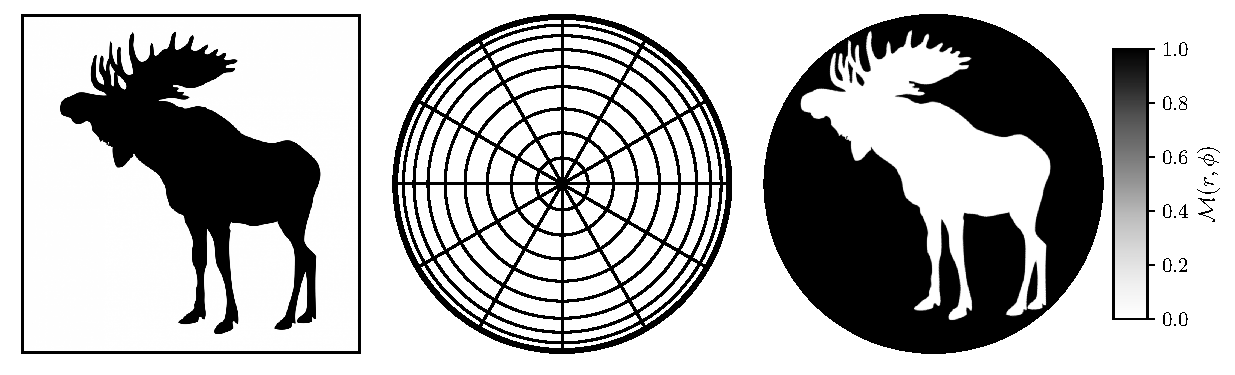
\includegraphics[width=\textwidth]{paper_figure01.pdf}
    \caption{ 
        (Left) A public-domain silhouette of a moose.
        (Middle) A sparse representation of the polar-coordinate grid on which we represent fields in our simulation.
        (Right) The Moosinesq mask $\mathcal{M}$ felt by our equations; fluid motions are damped where $\mathcal{M} > 0$.
        \label{fig:methods}
    }
\end{figure*}
